%
% orthogonal.tex
%
% (c) 2021 Prof Dr Andreas Müller, OST Ostschweizer Fachhochschule
%
\section{Orthogonale Funktionenfamilien
\label{buch:orthogonalitaet:section:orthogonale-funktionen}}
\rhead{Orthogonale Funktionenfamilien}
Die Fourier-Theorie basiert auf der Idee, Funktionen durch 
Funktionenreihen mit Summanden zu bilden, die im Sinne eines
Skalarproduktes orthogonal sind, welches mit Hilfe eines Integrals
definiert sind.
Solche Funktionenfamilien treten jedoch auch als Lösungen von
Differentialgleichungen.
Besonders interessant wird die Situation, wenn die Funktionen 
Polynome sind.

%
% Skalarprodukt
%
\subsection{Skalarprodukt}
Der reelle Vektorraum $\mathbb{R}^n$ trägt das Skalarprodukt
\[
\langle\;\,,\;\rangle
\colon
\mathbb{R}^n \times \mathbb{R}^n \to \mathbb{R}
:
(x,y)\mapsto \langle x, y\rangle = \sum_{k=1}^n x_iy_k,
\]
welches viele interessante Anwendungen ermöglicht.
Eine orthonormierte Basis macht es zum Beispiel besonders leicht,
eine Zerlegung eines Vektors in dieser Basis zu finden.
In diesem Abschnitt soll zunächst an die Eigenschaften erinnert
werden, die zu einem nützlichen 

\subsubsection{Eigenschaften eines Skalarproduktes}
Das Skalarprodukt erlaubt auch, die Länge eines Vektors $v$
als $|v| = \sqrt{\langle v,v\rangle}$ zu definieren.
Dies funktioniert natürlich nur, wenn die Wurzel auch immer
definiert ist, d.~h.~das Skalarprodukt eines Vektors mit sich
selbst darf nicht negativ sein.
Dazu dient die folgende Definition.

\begin{definition}
Sei $V$ ein reeller Vektorraum.
Eine bilineare Abbildung
\[
\langle\;\,,\;\rangle
\colon
V\times V
\to
\mathbb{R}
:
(u,v) \mapsto \langle u,v\rangle.
\]
heisst {\em positiv definit}, wenn für alle Vektoren $v \in V$ mit
$v\ne 0 \Rightarrow \langle v,v\rangle > 0$ 
Die {\em Norm} eines Vektors $v$ ist
$|v|=\sqrt{\langle v,v\rangle}$.
\end{definition}

Damit man mit dem Skalarprodukt sinnvoll rechnen kann, ist ausserdem
erforderlich, dass es eine einfache Beziehung zwischen 
$\langle x,y\rangle$ und $\langle y,x\rangle$ gibt.

\begin{definition}
Ein {\em Skalarprodukt} auf einem reellen Vektorraum $V$ ist eine
positiv definite, symmetrische bilineare Abbildung
\[
\langle\;\,,\;\rangle
\colon
V\times V
\to
\mathbb{R}
:
(u,v) \mapsto \langle u,v\rangle.
\]
\end{definition}

Das Skalarprodukt $\langle u,v\rangle=u^tv$ auf dem Vektorraum 
$\mathbb{R}^n$ erfüllt die Definition ganz offensichtlich,
sie führt auf die Komponentendarstellung
\[
\langle u,v\rangle = u^tv = \sum_{k=1}^n u_iv_i.
\]
Weitere Skalarprodukte ergeben ergeben sich mit jeder symmetrischen,
positiv definiten Matrix $G$ und der Definition
$\langle u,v\rangle_G=u^tGv$.
Ein einfacher Spezialfall tritt auf, wenn $G$ eine Diagonalmatrix
$\operatorname{diag}(w_1,\dots,w_n)$
mit positiven Einträgen $w_i>0$ auf der Diagonalen ist.
In diesem Fall schreiben wir
\[
\langle u,v\rangle_w
=
u^t\operatorname{diag}(w_1,\dots,w_n)v
=
\sum_{k=1}^n u_iv_i\,w_i
\]
und nennen $\langle \;\,,\;\rangle_w$ das {\em gewichtete Skalarprodukt}
mit {\em Gewichten $w_i$}.

\subsubsection{Skalarprodukte auf Funktionenräumen}
Das Integral ermöglicht jetzt, ein Skalarprodukt auf dem reellen
Vektorraum der stetigen Funktionen auf einem Intervall zu definieren.

\begin{definition}
\label{buch:orthogonal:def:skalarprodukt}
Sei $V$ der reelle Vektorraum $C([a,b])$ der reellwertigen, stetigen
Funktion auf dem Intervall $[a,b]$.
Dann ist 
\[
\langle\;\,,\;\rangle
\colon
C([a,b]) \times C([a,b]) \to \mathbb{R}
:
(f,g) \mapsto \langle f,g\rangle = \int_a^b f(x)g(x)\,dx.
\]
ein Skalarprodukt.
\end{definition}

Die Definition ist offensichtlich symmetrisch in $f$ und $g$ und
aus den Eigenschaften des Integrals ist klar, dass das Produkt
bilinear ist:
\begin{align*}
\langle \lambda_1 f_1+\lambda_2f_2,g\rangle
&=
\int_a^b (\lambda_1f_(x) +\lambda_2f_2(x))g(x)\,dx
=
\lambda_1\int_a^b f_1(x) g(x)\,dx
+
\lambda_2\int_a^b f_2(x) g(x)\,dx
\\
&=
\lambda_1\langle f_1,g\rangle
+
\lambda_2\langle f_2,g\rangle.
\end{align*}
Ausserdem ist es positiv definit, denn wenn $f(x_0) \ne 0$ ist,
dann gibt es wegen der Stetigkeit von $f$ eine Umgebung
$U=[x_0-\varepsilon,x_0+\varepsilon]$, derart, dass $|f(x)| > \frac12|f(x_0)|$
ist für alle $x\in U$.
Somit ist das Integral
\[
\langle f,f\rangle
=
\int_a^b |f(x)|^2\,dx
\ge
\int_{x_0-\varepsilon}^{x_0+\varepsilon} |f(x)|^2\,dx
\ge
\int_{x_0-\varepsilon}^{x_0+\varepsilon} \frac14|f(x_0)|^2\,dx
=
\frac{1}{4}|f(x_0)|^2\cdot 2\varepsilon
=
\frac{|f(x_0)|^2\varepsilon}{2}
>0,
\]
was beweist, dass $\langle\;,\;\rangle$ positiv definit und damit
ein Skalarprodukt ist.

Die Definition kann noch etwas verallgemeinert werden, indem 
die Funktionswerte nicht überall auf dem Definitionsbereich 
gleich gewichtet werden. 

\begin{definition}
\label{buch:orthogonal:def:skalarproduktw}
Sei $w\colon [a,b]\to \mathbb{R}^+$ eine positive, stetige Funktion,
dann ist
\[
\langle\;\,,\;\rangle_w
\colon
C([a,b]) \times C([a,b]) \to \mathbb{R}
:
(f,g) \mapsto \langle f,g\rangle_w = \int_a^b f(x)g(x)\,w(x)\,dx.
\]
das {\em gewichtete Skalarprodukt} mit {\em Gewichtsfunktion $w(x)$}.
\end{definition}

\subsubsection{Gram-Schmidt-Orthonormalisierung}
In einem reellen Vektorraum $V$ mit Skalarprodukt $\langle\;\,,\;\rangle$
kann aus einer beleibigen Basis $b_1,\dots,b_n$ mit Hilfe des 
Gram-Schmidtschen Orthogonalisierungsverfahrens immer eine
orthonormierte Basis $\tilde{b}_1,\dots,\tilde{b}_n$ Basis
gewonnen werden.
Es stellt sicher, dass für alle $k\le n$ gilt
\[
\langle b_1,\dots,b_k\rangle
=
\langle \tilde{b}_1,\dots,\tilde{b}_k\rangle.
\]
Zur Vereinfachung der Formeln schreiben wir $v^0=v/|v|$ für einen zu
$v$ parallelen Einheitsvektor.
Die Vektoren $\tilde{b}_i$ können mit Hilfe der Formeln
\begin{align*}
\tilde{b}_1
&=
(b_1)^0
\\
\tilde{b}_2
&=
\bigl(
b_2
-
\langle \tilde{b}_1,b_2\rangle \tilde{b}_1
\bigr)^0
\\
\tilde{b}_3
&=
\bigl(
b_3
-
\langle \tilde{b}_1,b_3\rangle \tilde{b}_1
-
\langle \tilde{b}_2,b_3\rangle \tilde{b}_2
\bigr)^0
\\
&\;\vdots
\\
\tilde{b}_n
&=
\bigl(
b_n
-
\langle \tilde{b}_1,b_n\rangle \tilde{b}_1
-
\langle \tilde{b}_2,b_n\rangle \tilde{b}_2
-\dots
-
\langle \tilde{b}_{n-1},b_n\rangle \tilde{b}_{n-1}
\bigr)^0
\end{align*}
iterativ berechnet werden.
Dieses Verfahren lässt sich auch auf Funktionenräume anwenden.

Die Normierung ist nicht unbedingt nötig und manchmal unangenehm,
da die Norm unschöne Quadratwurzeln einführt.
Falls es genügt, eine orthogonale Basis zu finden, kann darauf
verzichtet werden, bei der Orthogonalisierung muss aber berücksichtigt
werden, dass die Vektoren $\tilde{b}_i$ jetzt nicht mehr Einheitslänge
haben.
Die Formeln
\begin{align*}
\tilde{b}_0
&=
b_0
\\
\tilde{b}_1
&=
b_1
-
\frac{\langle b_1,\tilde{b}_0\rangle}{\langle \tilde{b}_0,\tilde{b}_0\rangle}\tilde{b}_0
\\
\tilde{b}_2
&=
b_2
-
\frac{\langle b_2,\tilde{b}_0\rangle}{\langle \tilde{b}_0,\tilde{b}_0\rangle}\tilde{b}_0
-
\frac{\langle b_2,\tilde{b}_1\rangle}{\langle \tilde{b}_1,\tilde{b}_1\rangle}\tilde{b}_1
\\
&\;\vdots
\\
\tilde{b}_n
&=
b_n
-
\frac{\langle b_n,\tilde{b}_0\rangle}{\langle \tilde{b}_0,\tilde{b}_0\rangle}\tilde{b}_0
-
\frac{\langle b_n,\tilde{b}_1\rangle}{\langle \tilde{b}_1,\tilde{b}_1\rangle}\tilde{b}_1
-
\dots
-
\frac{\langle b_n,\tilde{b}_{n-1}\rangle}{\langle \tilde{b}_{n-1},\tilde{b}_{n-1}\rangle}\tilde{b}_{n-1}.
\end{align*}
berücksichtigen dies.

\subsubsection{Selbstadjungierte Operatoren und Eigenvektoren}
Symmetrische Matrizen spielen eine spezielle Rolle in der
endlichdimensionalen linearen Algebra, weil sie sich immer
mit einer orthonormierten Basis diagonalisieren lassen.
In der vorliegenden Situation undendlichdimensionaler Vektorräume
brauchen wir eine angepasste Definition.

\begin{definition}
Eine lineare Selbstabbildung $A\colon V\to V$
eines Vektorrraums mit Skalarprodukt
heisst {\em selbstadjungiert}, wenn für alle Vektoren $u,v\in V$
heisst $\langle Au,v\rangle = \langle u,Av\rangle$.
\end{definition}

Es ist wohlbekannt, dass Eigenvektoren einer symmetrischen Matrix
zu verschiedenen Eigenwerten orthogonal sind.
Der Beweis ist direkt übertragbar, wir halten das Resultat hier
für spätere Verwendung fest.

\begin{satz}
Sind $f$ und $g$ Eigenvektoren eines selbstadjungierten Operators $A$
zu verschiedenen Eigenwerten $\lambda$ und $\mu$, dann sind $f$ und $g$
orthogonal.
\end{satz}

\begin{proof}[Beweis]
Im vorliegenden Zusammenhang möchten wir die Eigenschaft nutzen,
dass Eigenfunktionen eines selbstadjungierten Operatores zu verschiedenen
Eigenwerten orthogonal sind.
Dazu seien $Df = \lambda f$ und $Dg=\mu g$ und wir rechnen
\begin{equation*}
\renewcommand{\arraycolsep}{2pt}
\begin{array}{rcccrl}
\langle Df,g\rangle &=& \langle \lambda f,g\rangle &=& \lambda\phantom{)}\langle f,g\rangle
&\multirow{2}{*}{\hspace{3pt}$\biggl\}\mathstrut-\mathstrut$}\\
=\langle f,Dg\rangle &=& \langle f,\mu g\rangle &=& \mu\phantom{)}\langle f,g\rangle&
\\[2pt]
\hline
         0           & &                        &=& (\lambda-\mu)\langle f,g\rangle&
\end{array}
\end{equation*}
Da $\lambda-\mu\ne 0$ ist, muss $\langle f,g\rangle=0$ sein.
\end{proof}

\begin{beispiel}
Sei $C^1([0,2\pi], \mathbb{C})=C^1(S^1,\mathbb{C})$
der Vektorraum der $2\pi$-periodischen differenzierbaren Funktionen mit
dem Skalarprodukt 
\[
\langle f,g\rangle
=
\frac{1}{2\pi}\int_0^{2\pi} \overline{f(t)}g(t)\,dt
\]
enthält die Funktionen $e_n(t) = e^{int}$.
Der Operator
\[
D=i\frac{d}{dt}
\]
ist selbstadjungiert, denn mit Hilfe von partieller Integration erhält man
\[
\langle Df,g\rangle
=
\frac{1}{2\pi}
\int_0^{2\pi}
\underbrace{
\overline{i\frac{df(t)}{dt}}
}_{\uparrow}
\underbrace{g(t)}_{\downarrow}
\,dt
=
\underbrace{
\frac{-i}{2\pi}
\biggl[
\overline{f(t)}g(t)
\biggr]_0^{2\pi}
}_{\displaystyle=0}
+
\frac{1}{2\pi}
\int_0^{2\pi}
\overline{f(t)}i\frac{dg(t)}{dt}
\,dt
=
\langle f,Dg\rangle
\]
unter Ausnützung der $2\pi$-Periodizität der Funktionen.

Die Funktionen $e_n(t)$ sind Eigenfunktionen des Operators $D$, denn
\[
De_n(t) = i\frac{d}{dt}e^{int} = -n e^{int} = -n e_n(t).
\]
Nach obigem Satz sind die Eigenfunktionen von $D$ orthogonal.
\end{beispiel}

Das Beispiel illustriert, dass orthogonale Funktionenfamilien
ein automatisches Nebenprodukt selbstadjungierter Operatoren sind.


% XXX Orthogonalisierungsproblem so formulieren, dass klar wird,
% XXX dass man ein "Normierungskriterium braucht.

Da wir auf die Normierung verzichten, brauchen wir ein anderes
Kriterium, welches die Polynome eindeutig festlegen kann.
Wir bezeichnen das Polynom vom Grad $n$, das bei diesem Prozess
entsteht, mit $P_n(x)$ und legen willkürlich aber traditionskonform
fest, dass $P_n(1)=1$ sein soll.

Das Skalarprodukt berechnet ein Integral eines Produktes von zwei
Polynomen über das symmetrische Interval $[-1,1]$.
Ist die eine gerade und die andere ungerade, dann ist das
Produkt eine ungerade Funktion und das Skalarprodukt verschwindet.
Sind beide Funktionen gerade oder ungerade, dann ist das Produkt
gerade und das Skalarprodukt ist im Allgmeinen von $0$ verschieden.
Dies zeigt, dass es tatsächlich etwas zu Orthogonalisieren gibt.

Die ersten beiden Funktionen sind das konstante Polynom $1$ und
das Polynome $x$.
Nach obiger Beobachtung ist das Skalarprodukt $\langle 1,x\rangle=0$,
also ist $P_1(x)=x$.
Die Graphen der entstehenden Polynome sind in
Abbildung~\ref{buch:integral:orthogonal:legendregraphen}
dargestellt.
\begin{figure}
\centering
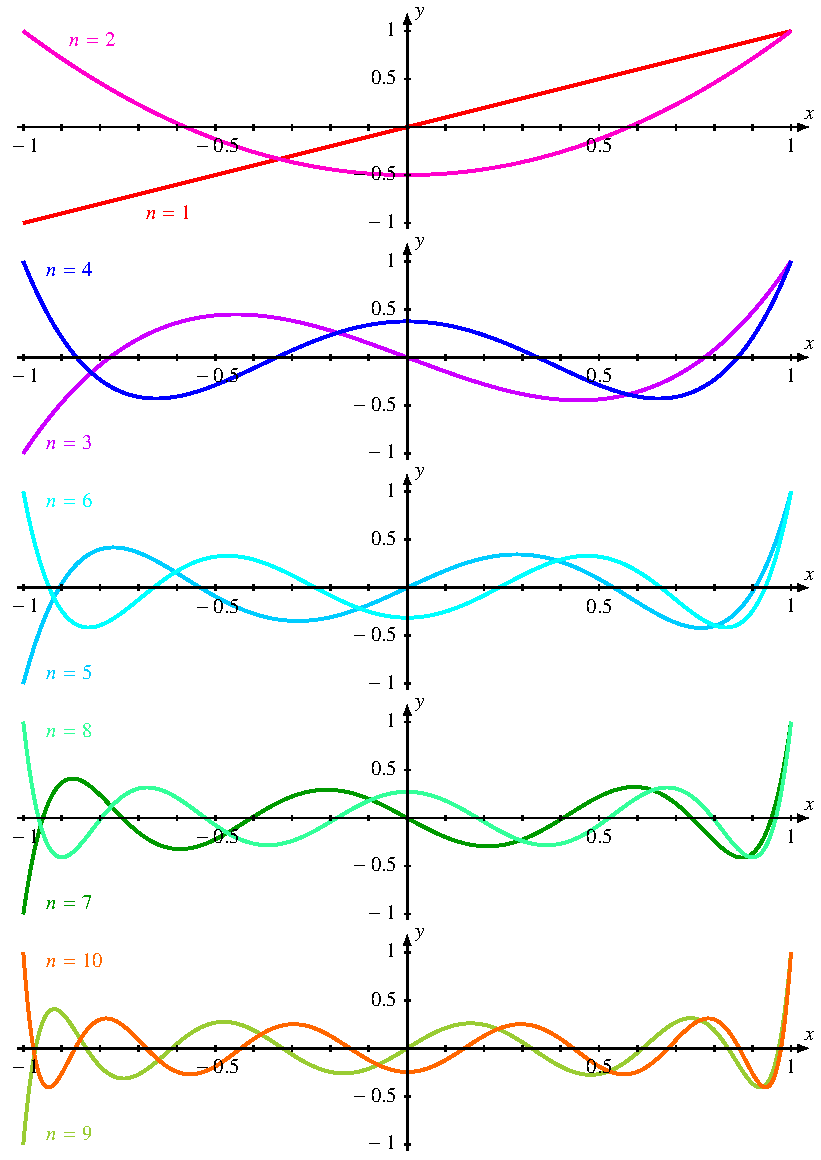
\includegraphics{chapters/070-orthogonalitaet/images/legendre.pdf}
\caption{Graphen der Legendre-Polynome $P_n(x)$ für $n=1,\dots,10$.
\label{buch:integral:orthogonal:legendregraphen}}
\end{figure}

\begin{lemma}
Die Polynome $P_{2n}(x)$ sind gerade, die Polynome $P_{2n+1}(x)$ sind
ungerade Funktionen von $x$.
\end{lemma}

\begin{proof}[Beweis]
Wir verwenden vollständige Induktion nach $n$.
Wir wissen bereits, dass $P_0(x)=1$ und $P_1(x)=x$ die verlangten
Symmetrieeigenschaften haben.
Im Sinne der Induktionsannahme nehmen wir daher an, dass die
Symmetrieeigenschaften für $P_k(x)$, $k<n$, bereits bewiesen sind.
$P_n(x)$ entsteht jetzt durch Orthogonalisierung nach der Formel
\[
P_n(x)
=
x^n
-
\langle P_{n-1},x^n\rangle P_{n-1}(x)
-
\langle P_{n-2},x^n\rangle P_{n-2}(x)
-\dots-
\langle P_1,x^n\rangle P_1(x)
-
\langle P_0,x^n\rangle P_0(x).
\]
Die Skalarprodukte
$\langle P_{n-1},x^n\rangle$,
$\langle P_{n-3},x^n\rangle$, $\dots$ verschwinden alle, so dass
$P_n(x)$ eine Linearkombination der Funktionen $x^n$, $P_{n-2}(x)$,
$P_{n-4}(x)$ ist, die die gleiche Parität wie $x^n$ haben.
Also hat auch $P_n(x)$ die gleiche Parität, was das Lemma beweist.
\end{proof}

Die Ortogonalisierung von $x^2$ liefert daher
\[
p(x) = x^2
-
\frac{\langle x^2,P_0\rangle}{\langle P_0,P_0\rangle} P_0(x)
=
x^2 - \frac{\int_{-1}^1x^2\,dx}{\int_{-1}^11\,dx}
=
x^2 - \frac{\frac{2}{3}}{2}=x^2-\frac13
\]
Dieses Polynom erfüllt die Standardisierungsbedingung noch 
nicht den $p(1)=\frac23$.
Daraus leiten wir ab, dass
\[
P_2(x) = \frac12(3x^2-1)
\]
ist.

Für $P_3(x)$ brauchen wir nur die Skalaprodukte
\[
\left.
\begin{aligned}
\langle x^3,P_1\rangle
&=
\int_{-1}^1  x^3\cdot x\,dx
=
\biggl[\frac15x^5\biggr]_{-1}^1
=
\frac25
\qquad
\\
\langle P_1,P_1\rangle
&=
\int_{-1}^1 x^2\,dx
=
\frac23
\end{aligned}
\right\}
\qquad
\Rightarrow
\qquad
p(x) = x^3 - \frac{\frac25}{\frac23}x=x^3-\frac{3}{5}x
\]
Die richtige Standardisierung ergibt sich,
indem man durch $p(1)=\frac25$ dividiert, also
\[
P_2(x) = \frac12(5x^3-3x).
\]

Die Berechnung weiterer Polynome verlangt, dass Skalarprodukte
$\langle x^n,P_k\rangle$ berechnet werden müssen, was wegen
der zunehmend komplizierten Form von $P_k$ etwas mühsam ist.
Wir berechnen den Fall $P_4$.
Dazu muss das Polynom $x^4$ um eine Linearkombination von
$P_2$ und $P_0(x)=1$ korrigiert werden.
Die Skalarprodukte sind
\begin{align*}
\langle x^4, P_0\rangle
&=
\int_{-1}^1 x^4\,dx = \frac25
\\
\langle P_0,P_0\rangle
&=
\int_{-1}^1 \,dx = 2
\\
\langle x^4,P_2\rangle
&=
\int_{-1}^1 \frac32x^6-\frac12 x^4\,dx
=
\biggl[\frac{3}{14}x^7-\frac{1}{10}x^5\biggr]_{-1}^1
=
\frac6{14}-\frac15
=
\frac8{35}
\\
\langle P_2,P_2\rangle
&=
\int_{-1}^1 \frac14(3x^2-1)^2\,dx
=
\int_{-1}^1 \frac14(9x^4-6x^2+1)\,dx
=
\frac14(\frac{18}{5}-4+2)
=\frac25.
\end{align*}
Daraus folgt für $p(x)$
\begin{align*}
p(x)
&=
x^4
-
\frac{\langle x^4,P_2\rangle}{\langle P_2,P_2\rangle}P_2(x)
-
\frac{\langle x^4,P_0\rangle}{\langle P_0,P_0\rangle}P_0(x)
\\
&=
x^4
-\frac47 P_2(x) - \frac15 P_0(x)
\\
&=
x^4 - \frac{6}{7}x^2 + \frac{3}{35}
\end{align*}
mit $p(1)=\frac{8}{35}$, so dass man
\[
P_4(x) =
\frac18(35x^4-30x^2+3)
\]
setzen muss.

\begin{figure}
\centering
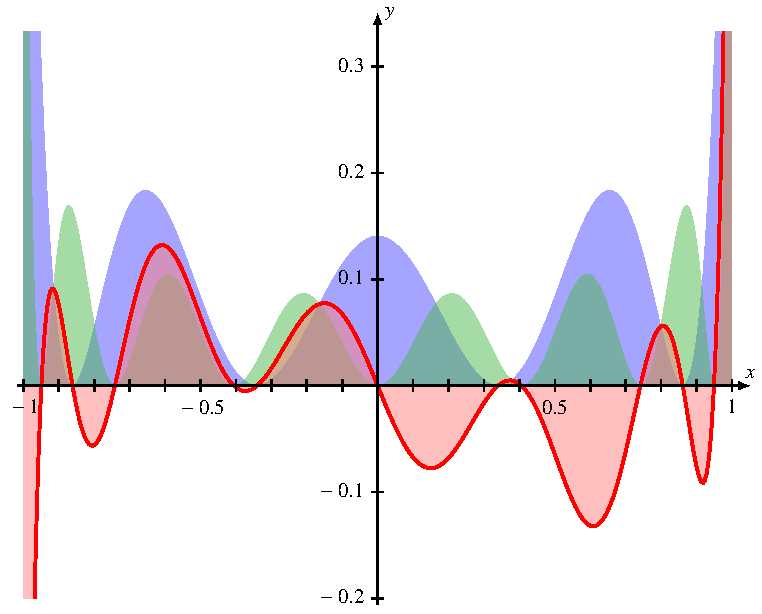
\includegraphics{chapters/070-orthogonalitaet/images/orthogonal.pdf}
\caption{Orthogonalität der Legendre-Polynome $P_4(x)$ ({\color{blue}blau})
und $P_7(x)$ ({\color{darkgreen}grün}).
Die blaue Fläche ist die Fläche unter dem Graphen 
von $P_4(x)^2$, $P_4(x)$ muss durch die Wurzel aus diesem Flächeninhalt
geteilt werden, um ein Polynome mit Norm $1$ zu erhalten.
Für die grüne Fläche ist es $P_7(x)$.
Die rote Kurve ist der Graph der Funktion $P_4(x)\cdot P_7(x)$,
die rote Fläche ist deren Integral, sie ist $0$, d.~h.~die beiden
Funktionen sind orthogonal.
\label{buch:integral:orthogonal:legendreortho}}
\end{figure}

\begin{table}
\centering
\renewcommand{\arraystretch}{1.2}
\begin{tabular}{|>{$}c<{$}|>{$}l<{$}|}
\hline
n&P_n(x)\\
\hline
 0&1
\\
 1&x
\\
 2&\frac12(3x^2-1)
\\
 3&\frac12(5x^3-3x)
\\
 4&\frac18(35x^4-30x^2+3)
\\
 5&\frac18(63x^5-70x^3+15x)
\\
 6&\frac1{16}(231x^6-315x^4+105x^2-5)
\\
 7&\frac1{16}(429x^7-693x^5+315x^3-35x)
\\
 8&\frac1{128}(6435x^8-12012x^6+6930x^4-1260x^2+35)
\\
 9&\frac1{128}(12155x^9-25740x^7+18018x^5-4620x^3+315x)
\\
10&\frac1{256}(46189x^{10}-109395x^8+90090x^6-30030x^4+3465x^2-63)
\\[2pt]
\hline
\end{tabular}
\caption{Die Legendre-Polynome $P_n(x)$ für $n=0,1,\dots,10$ sind
orthogonale Polynome vom Grad $n$, die den Wert $P_n(1)=1$ haben.
\label{buch:integral:table:legendre-polynome}}
\end{table}

Die so konstruierten Polynome heissen die {\em Legendre-Polynome}.
Durch weitere Durchführung des Verfahrens liefert die Polynome in
Tabelle~\ref{buch:integral:table:legendre-polynome}.
Die Graphen sind in Abbildung~\ref{buch:integral:orthogonal:legendregraphen}
dargestellt.
Abbildung~\ref{buch:integral:orthogonal:legendreortho} illustriert, 
dass die die beiden Polynome $P_4(x)$ und $P_7(x)$ orthogonal sind.
Das Produkt $P_4(x)\cdot P_7(x)$ hat Integral $=0$.

%
% Rekursionsrelation
%
\subsection{Drei-Term-Rekursion
\label{buch:orthogonal:subsection:rekursionsrelation}}
Die Berechnung der Legendre-Polynome mit Hilfe des Gram-Schmidt-Verfahrens
ist ausserordentlich mühsame wenig hilfreich, wenn es darum geht, Werte
der Polynome zu berechnen.
Glücklicherweise erfüllen orthogonale Polynome automatisch eine 
Rekursionsbeziehung mit nur drei Termen.
Zum Beispiel kann man zeigen, dass für die Legendre-Polynome die
Relation
\begin{align*}
nP_n(x) &= (2n-1)xP_{n-1}(x) - (n-1)P_{n-2}(x),\;\forall n\ge 2,
\\
P_1(x) &= x,
\\
P_0(x) &= 1.
\end{align*}
Mit so einer Rekursionsbeziehung ist es sehr einfach, die Funktionswerte
für alle $P_n(x)$ zu berechnen.

\begin{definition}
Eine Folge von Polynomen $p_n(x)$ heisst orthogonal bezüglich des
Skalarproduktes $\langle\,\;,\;\rangle_w$, wenn 
\[
\langle p_n,p_m\rangle_w = h_n \delta_{nm}
\]
für alle $n$, $m$.
\end{definition}

\subsubsection{Allgemeine Drei-Term-Rekursion für orthogonale Polynome}
Der folgende Satz besagt, dass $p_n$ eine Rekursionsbeziehung erfüllt.

\begin{satz}
\label{buch:orthogonal:satz:drei-term-rekursion}
Eine Folge bezüglich $\langle\,\;,\;\rangle_w$ orthogonaler Polynome $p_n$ 
mit dem Grade $\deg p_n = n$ erfüllt eine Rekursionsbeziehung der Form
\begin{equation}
p_{n+1}(x)
=
(A_nx+B_n)p_n(x) - C_np_{n-1}(x)
\label{buch:orthogonal:eqn:rekursion}
\end{equation}
für $n\ge 0$, wobei $p_{-1}(x)=0$ gesetzt wird.
Die Zahlen $A_n$, $B_n$ und $C_n$ sind reell und es ist
$A_{n-1}A_nC_n\ge 0$ für $n>0$. 
Wenn $k_n>0$ der Leitkoeffizient von $p_n(x)$ ist, dann gilt
\begin{equation}
A_n=\frac{k_{n+1}}{k_n},
\qquad
C_{n+1} = \frac{A_{n+1}}{A_n}\frac{h_{n+1}}{h_n}.
\label{buch:orthogonal:eqn:koeffizientenrelation}
\end{equation}
\end{satz}

\subsubsection{Multiplikationsoperator mit $x$}
Man kann die Relation auch nach dem Produkt $xp_n(x)$ auflösen, dann
wird sie
\begin{equation}
xp_n(x)
=
\frac{1}{A_n}p_{n+1}(x)
-
\frac{B_n}{A_n}p_n(x)
+
\frac{C_n}{A_n}p_{n-1}(x).
\label{buch:orthogonal:eqn:multixrelation}
\end{equation}
Die Multiplikation mit $x$ ist eine lineare Abbildung im Raum der Funktionen.
Die Relation~\eqref{buch:orthogonal:eqn:multixrelation} besagt, dass diese
Abbildung in der Basis der Polynome $p_k$ tridiagonale Form hat.

\subsubsection{Drei-Term-Rekursion für die Tschebyscheff-Polynome}
Eine Relation der Form~\eqref{buch:orthogonal:eqn:multixrelation}
wurde bereits in 
Abschnitt~\ref{buch:potenzen:tschebyscheff:rekursionsbeziehungen}
hergeleitet.
In der Form~\eqref{buch:orthogonal:eqn:rekursion} geschrieben lautet
sie
\[
T_{n+1}(x) = 2x\,T_n(x)-T_{n-1}(x).
\]
also
$A_n=2$, $B_n=0$ und $C_n=1$.

\subsubsection{Beweis von Satz~\ref{buch:orthogonal:satz:drei-term-rekursion}}
Die Relation~\eqref{buch:orthogonal:eqn:multixrelation} zeigt auch,
dass der Beweis die Koeffizienten $\langle xp_k,p_j\rangle_w$
berechnen muss.
Dabei wird wiederholt der folgende Trick verwendet.
Für jede beliebige Funktion $f$ mit $\|f\|_w^2<\infty$ ist
\[
\langle fp_k,p_j\rangle_w
=
\langle p_k,fp_j\rangle_w.
\]
Für $f(x)=x$ kann man weiter verwenden, dass $xp_k(x)$ ein Polynom
vom Grad $k+1$ ist.
Die Gleichheit $\langle xp_k,p_j\rangle_w=\langle p_k,xp_j\rangle_w$
ermöglicht also, den Faktor $x$ dorthin zu schieben, wo es nützlicher ist.

\begin{proof}[Beweis des Satzes]
Multipliziert man die rechte Seite von
\eqref{buch:orthogonal:eqn:rekursion} aus, dann ist der einzige Term
vom Grad $n+1$ der Term $A_nxp_n(x)$.
Der Koeffizient $A_n$ ist also dadurch festgelegt, dass
\begin{equation}
b(x)
=
p_{n+1}(x) - A_nxp_n(x)
\label{buch:orthogonal:rekbeweis}
\end{equation}
Grad $\le n$ hat.
Dazu müssen sich die Terme vom Grad $n+1$ in den Polynomen wegheben,
d.~h.~$k_{n+1}-A_nk_n=0$, woraus die erste Beziehung in
\eqref{buch:orthogonal:eqn:koeffizientenrelation} folgt.

Die Polynome $p_k$ sind durch Orthogonalisierung der Monome
$1$, $x$,\dots $x^{k}$ entstanden.
Dies bedeutet, dass $\langle p_n,x^k\rangle_w=0$ für alle $k<n$
gilt und daher auch $\langle p_n,Q\rangle_w=0$ für jedes Polynome
$Q(x)$ vom Grad $<n$.

Das Polynom $b(x)$ ist vom Grad $\le n$, es lässt sich also als
Linearkombination
\[
b(x) = \sum_{k=0}^n b_k p_k(x)
\]
der $p_k$ mit $k\le n$ schreiben.
Die Koeffizienten $b_j$ kann man erhalten, indem man 
\eqref{buch:orthogonal:rekbeweis} Skalar mit $p_j$ multipliziert.
Dabei erhält man
\[
h_jb_j
=
\langle b,p_j\rangle_w
=
\langle p_{n+1},p_j\rangle_w
-
A_n\langle xp_n,p_j\rangle_w.
\]
Für $j\le n$ verschwindet der erste Term nach der Definition einer
Folge von orthogonalen Polynomen.
Den zweiten Term kann man umformen in
\[
\langle xp_n,p_j\rangle_w
=
\langle p_n,xp_j\rangle_w.
\]
Darin ist $xp_j$ ein Polynom vom Grad $j+1$.
Für $n>j+1$ folgt, dass der zweite Term verschwindet.
Somit sind alle $b_j=0$ mit $j<n-1$, nur der Term $j=n-1$
bleibt bestehen.
Mit $B_n=b_n$ und $C_n=b_{n-1}$ bekommt man die somit die
Rekursionsbeziehung~\eqref{buch:orthogonal:eqn:rekursion}.

Indem man das Skalarprodukt von~\eqref{buch:orthogonal:eqn:rekursion}
mit $p_{n-1}$ bildet, findet man
\begin{align}
\underbrace{\langle
p_{n+1},p_{n-1}
\rangle_w}_{\displaystyle=0}
&=
\langle (A_nx+B_n)p_n+C_np_{n-1},p_{n-1} \rangle_w
\notag
\\
0
&=
A_n\langle xp_n,p_{n-1} \rangle_w
+B_n\underbrace{\langle p_n,b_{n-1}\rangle_w}_{\displaystyle=0}
-C_n\|p_{n-1}\|_w^2
\notag
\\
0
&=
A_n\langle p_n,xp_{n-1} \rangle_w
-C_n\|p_{n-1}\|_w^2
\label{buch:orthogonal:eqn:rekbeweis2}
\end{align}
Indem man $xp_n$ als
\[
xp_{n-1}(x)
=
\frac{k_{n-1}}{k_n} p_n(x)
+
\sum_{k=0}^{n-1} d_kp_k(x)
\]
schreibt, bekommt man
\begin{align*}
\langle
p_n,
xp_{n-1}
\rangle_w
&=
\biggl\langle
p_n,
\frac{k_{n-1}}{k_n} p_n
+
\sum_{k=0}^{n-1} d_kp_k
\biggr\rangle_w
=
\frac{k_{n-1}}{k_n}h_n
+
\sum_{k=0}^{n-1} d_k\underbrace{\langle p_n,p_k\rangle_w}_{\displaystyle=0}
\end{align*}
Eingesetzt in~\eqref{buch:orthogonal:eqn:rekbeweis2} erhält man
\[
A_n\frac{k_{n-1}}{k_n}h_n = C_n h_{n-1}
\qquad\Rightarrow\qquad
C_n
=
A_n\frac{k_{n-1}}{k_n}\frac{h_n}{h_{n-1}},
\]
damit ist auch die zweite Beziehung von
\eqref{buch:orthogonal:eqn:koeffizientenrelation}.
\end{proof}
